	% uWaterloo Thesis Template for LaTeX 
% Last Updated May 24, 2011 by Stephen Carr, IST Client Services
% FOR ASSISTANCE, please send mail to rt-IST-CSmathsci@ist.uwaterloo.ca

% Effective October 2006, the University of Waterloo 
% requires electronic thesis submission. See the uWaterloo thesis regulations at
% http://www.grad.uwaterloo.ca/Thesis_Regs/thesistofc.asp.

% DON'T FORGET TO ADD YOUR OWN NAME AND TITLE in the "hyperref" package
% configuration below. THIS INFORMATION GETS EMBEDDED IN THE PDF FINAL PDF DOCUMENT.
% You can view the information if you view Properties of the PDF document.

% Many faculties/departments also require one or more printed
% copies. This template attempts to satisfy both types of output. 
% It is based on the standard "book" document class which provides all necessary 
% sectioning structures and allows multi-part theses.

% DISCLAIMER
% To the best of our knowledge, this template satisfies the current uWaterloo requirements.
% However, it is your responsibility to assure that you have met all 
% requirements of the University and your particular department.
% Many thanks to the feedback from many graduates that assisted the development of this template.

% -----------------------------------------------------------------------

% By default, output is produced that is geared toward generating a PDF 
% version optimized for viewing on an electronic display, including 
% hyperlinks within the PDF.
 
% E.g. to process a thesis called "mythesis.tex" based on this template, run:

% pdflatex mythesis	-- first pass of the pdflatex processor
% bibtex mythesis	-- generates bibliography from .bib data file(s) 
% pdflatex mythesis	-- fixes cross-references, bibliographic references, etc
% pdflatex mythesis	-- fixes cross-references, bibliographic references, etc

% If you use the recommended LaTeX editor, Texmaker, you would open the mythesis.tex
% file, then click the pdflatex button. Then run BibTeX (under the Tools menu).
% Then click the pdflatex button two more times. If you have an index as well,
% you'll need to run MakeIndex from the Tools menu as well, before running pdflatex
% the last two times.

% N.B. The "pdftex" program allows graphics in the following formats to be
% included with the "\includegraphics" command: PNG, PDF, JPEG, TIFF
% Tip 1: Generate your figures and photos in the size you want them to appear
% in your thesis, rather than scaling them with \includegraphics options.
% Tip 2: Any drawings you do should be in scalable vector graphic formats:
% SVG, PNG, WMF, EPS and then converted to PNG or PDF, so they are scalable in
% the final PDF as well.
% Tip 3: Photographs should be cropped and compressed so as not to be too large.

% To create a PDF output that is optimized for double-sided printing: 
%
% 1) comment-out the \documentclass statement in the preamble below, and
% un-comment the second \documentclass line.
%
% 2) change the value assigned below to the boolean variable
% "PrintVersion" from "false" to "true".

% --------------------- Start of Document Preamble -----------------------

% Specify the document class, default style attributes, and page dimensions
% For hyperlinked PDF, suitable for viewing on a computer, use this:
\documentclass[letterpaper,12pt,titlepage,oneside,final]{book}
 
% For PDF, suitable for double-sided printing, change the PrintVersion variable below
% to "true" and use this \documentclass line instead of the one above:
%\documentclass[letterpaper,12pt,titlepage,openright,twoside,final]{book}

% Some LaTeX commands I define for my own nomenclature.
% If you have to, it's better to change nomenclature once here than in a 
% million places throughout your thesis!
\newcommand{\package}[1]{\textbf{#1}} % package names in bold text
\newcommand{\cmmd}[1]{\textbackslash\texttt{#1}} % command name in tt font 
\newcommand{\href}[1]{#1} % does nothing, but defines the command so the
    % print-optimized version will ignore \href tags (redefined by hyperref pkg).
%\newcommand{\texorpdfstring}[2]{#1} % does nothing, but defines the command
% Anything defined here may be redefined by packages added below...

% This package allows if-then-else control structures.
\usepackage{ifthen}
\newboolean{PrintVersion}
\setboolean{PrintVersion}{false} 
\usepackage{caption}
\captionsetup{skip=8pt}
% CHANGE THIS VALUE TO "true" as necessary, to improve printed results for hard copies
% by overriding some options of the hyperref package below.

%\usepackage{nomencl} % For a nomenclature (optional; available from ctan.org)
\pdfoptionpdfminorversion 6
\usepackage{amsmath,amssymb,amstext,natbib, verbatim} % Lots of math symbols and environments
\usepackage[pdftex]{graphicx} % For including graphics N.B. pdftex graphics driver 
\usepackage[pdftex,letterpaper=true,pagebackref=false]{hyperref} % with basic options
\usepackage[latin1]{inputenc}
\usepackage{tikz}
\usepackage{geometry,setspace,datetime}
\usetikzlibrary{shapes,arrows}
% for the definitions
\usepackage{amsthm}
\newtheorem{lemma}{Lemma}[section]
\newtheorem{theorem}[lemma]{Theorem}
\newtheorem{corollary}[lemma]{Corollary}
\newtheorem{conjecture}[lemma]{Conjecture}
\newtheorem{proposition}[lemma]{Proposition}
\newtheorem{remark}[lemma]{Remark}
\newtheorem{definition}[lemma]{Definition}
\newtheorem{example}[lemma]{Example}


%testing placement
\usepackage{float}% If comment this, figure moves to Page 2
\usepackage{lipsum}

		
\hypersetup{
    plainpages=false,       % needed if Roman numbers in frontpages
    pdfpagelabels=true,     % adds page number as label in Acrobat's page count
    bookmarks=true,         % show bookmarks bar?
    unicode=false,          % non-Latin characters in Acrobat’s bookmarks
    pdftoolbar=true,        % show Acrobat’s toolbar?
    pdfmenubar=true,        % show Acrobat’s menu?
    pdffitwindow=false,     % window fit to page when opened
    pdfstartview={FitH},    % fits the width of the page to the window
    pdftitle={uWaterloo\ LaTeX\ Thesis\ Template},    % title: CHANGE THIS TEXT!
%    pdfauthor={Author},    % author: CHANGE THIS TEXT! and uncomment this line
%    pdfsubject={Subject},  % subject: CHANGE THIS TEXT! and uncomment this line
%    pdfkeywords={keyword1} {key2} {key3}, % list of keywords, and uncomment this line if desired
    pdfnewwindow=true,      % links in new window
    colorlinks=true,        % false: boxed links; true: colored links
    linkcolor=blue,         % color of internal links
    citecolor=blue,        % color of links to bibliography
    filecolor=magenta,      % color of file links
    urlcolor=blue           % color of external links
}
\ifthenelse{\boolean{PrintVersion}}{   % for improved print quality, change some hyperref options
\hypersetup{	% override some previously defined hyperref options
%    colorlinks,%
    citecolor=black,%
    filecolor=black,%
    linkcolor=black,%
    urlcolor=black}
}{} % end of ifthenelse (no else)

% Setting up the page margins...
% uWaterloo thesis requirements specify a minimum of 1 inch (72pt) margin at the
% top, bottom, and outside page edges and a 1.125 in. (81pt) gutter
% margin (on binding side). While this is not an issue for electronic
% viewing, a PDF may be printed, and so we have the same page layout for
% both printed and electronic versions, we leave the gutter margin in.
% Set margins to minimum permitted by uWaterloo thesis regulations:
\setlength{\marginparwidth}{0pt} % width of margin notes
% N.B. If margin notes are used, you must adjust \textwidth, \marginparwidth
% and \marginparsep so that the space left between the margin notes and page
% edge is less than 15 mm (0.6 in.)
\setlength{\marginparsep}{0pt} % width of space between body text and margin notes
\setlength{\evensidemargin}{0.125in} % Adds 1/8 in. to binding side of all 
% even-numbered pages when the "twoside" printing option is selected
\setlength{\oddsidemargin}{0.125in} % Adds 1/8 in. to the left of all pages
% when "oneside" printing is selected, and to the left of all odd-numbered
% pages when "twoside" printing is selected
\setlength{\textwidth}{6.375in} % assuming US letter paper (8.5 in. x 11 in.) and 
% side margins as above
\raggedbottom

% The following statement specifies the amount of space between
% paragraphs. Other reasonable specifications are \bigskipamount and \smallskipamount.
\setlength{\parskip}{\medskipamount}

% The following statement controls the line spacing.  The default
% spacing corresponds to good typographic conventions and only slight
% changes (e.g., perhaps "1.2"), if any, should be made.
\renewcommand{\baselinestretch}{1.7} % this is the default line space setting

% By default, each chapter will start on a recto (right-hand side)
% page.  We also force each section of the front pages to start on 
% a recto page by inserting \cleardoublepage commands.
% In many cases, this will require that the verso page be
% blank and, while it should be counted, a page number should not be
% printed.  The following statements ensure a page number is not
% printed on an otherwise blank verso page.
\let\origdoublepage\cleardoublepage
\newcommand{\clearemptydoublepage}{%
  \clearpage{\pagestyle{empty}\origdoublepage}}
\let\cleardoublepage\clearemptydoublepage

%======================================================================
%   L O G I C A L    D O C U M E N T -- the content of your thesis
%======================================================================
\begin{document}


% For a large document, it is a good idea to divide your thesis
% into several files, each one containing one chapter.
% To illustrate this idea, the "front pages" (i.e., title page,
% declaration, borrowers' page, abstract, acknowledgements,
% dedication, table of contents, list of tables, list of figures,
% nomenclature) are contained within the file "uw-ethesis-frontpgs.tex" which is
% included into the document by the following statement.
%----------------------------------------------------------------------
% FRONT MATERIAL
%----------------------------------------------------------------------


% T I T L E   P A G E
% -------------------
% Last updated May 24, 2011, by Stephen Carr, IST-Client Services
% The title page is counted as page `i' but we need to suppress the
% page number.  We also don't want any headers or footers.

% Example LaTeX source file suitable for producing output in PDF
%\documentclass[10pt]{report}
%\usepackage[pdftex]{graphicx}
%\usepackage{rotating,cite}

%\usepackage[pdftex]{hyperref} % This pkg should always be added last 
%\begin{document}
%\chapter{Example Photograph} 
%\begin{figure}
%\label{myfig}
%\begin{center}
%\includegraphics[clip=true,width=4in,height=3in]{myphoto.jpg}
%\end{center}
%\caption{My Photograph}
%\end{figure}
%\chapter{Example Sideways Table}
%\begin{sidewaystable}
%\label{mytable}
% table code goes here
%\caption{My Sideways Table and Caption}
%\end{sidewaystable}


\pagestyle{empty}
\pagenumbering{roman}

% The contents of the title page are specified in the "titlepage"
% environment.
\begin{titlepage}
        \begin{center}
        \vspace*{0.5cm}

        \Huge
        {\bf  Negotiations  Support System with Third Party Intervention}

        \vspace*{0.5cm}

        \normalsize
        by \\

        \vspace*{0.5cm}

        \Large
        Rami Abdulraheem A. Kinsara \\
        	%\vspace*{0.5cm}
	%\normalsize Supervisors: Professor Keith W. Hipel, and Professor D. Marc Kilgour
        \vspace*{0.5cm}

        \normalsize
        A thesis \\
        presented to the University of Waterloo \\ 
        in fulfillment of the \\
        thesis requirement for the degree of \\
        Doctor of Philosophy \\
        in \\
        Systems Design Engineering \\

        \vspace*{0.5cm}

        Waterloo, Ontario, Canada, 2014 \\

        \vspace*{0.5cm}

        \copyright\ Rami Abdulraheem A. Kinsara 2013 \\
        
        \vspace{0.5cm}
        
	%\today    
	     
        \end{center}
\end{titlepage}

% The rest of the front pages should contain no headers and be numbered using Roman numerals starting with `ii'
\pagestyle{plain}
\setcounter{page}{2}

\cleardoublepage % Ends the current page and causes all figures and tables that have so far appeared in the input to be printed.
% In a two-sided printing style, it also makes the next page a right-hand (odd-numbered) page, producing a blank page if necessary.
 


% D E C L A R A T I O N   P A G E
% -------------------------------
  % The following is the sample Delaration Page as provided by the GSO
  % December 13th, 2006.  It is designed for an electronic thesis.
 % \noindent
%I hereby declare that I am the sole author of this thesis. This is a true copy of the thesis, including any required final revisions, as accepted by my examiners.

  %\bigskip
  
 % \noindent
%I understand that my thesis may be made electronically available to the public.

%\cleardoublepage
%\newpage

% A B S T R A C T
% ---------------
\addcontentsline{toc}{chapter}{Abstract}
\begin{center}\textbf{Abstract}\end{center}

Systems methodologies to model third party mediation in international conflicts are developed within the framework of the Graph Model for Conflict Resolution (GMCR). The methodologies proposed give a better understanding of the conflict and how decision makers (DMs) can be motivated to undertake certain actions. The inverse approach to GMCR tackles the problem of specifying which preferences  for DMs lead to a particular resolution, making it easier for a mediator or other third party to influence the course of the conflict. The methodologies will be applied to real world conflicts, including a complex water conflict in the Middle East.

\cleardoublepage
%\newpage

% A C K N O W L E D G E M E N T S
% -------------------------------

%\begin{center}\textbf{Acknowledgements}\end{center}

%I would like to thank all the little people who made this possible.
%\cleardoublepage
%\newpage

% D E D I C A T I O N
% -------------------

%\begin{center}\textbf{Dedication}\end{center}

%This is dedicated to the one I love.
%\cleardoublepage
%\newpage

% T A B L E   O F   C O N T E N T S
% ---------------------------------
\renewcommand\contentsname{Table of Contents}
\tableofcontents
\cleardoublepage
\phantomsection
%\newpage

% L I S T   O F   T A B L E S
% ---------------------------
%\addcontentsline{toc}{chapter}{List of Tables}
%\listoftables
%\cleardoublepage
%\phantomsection		% allows hyperref to link to the correct page
%\newpage

% L I S T   O F   F I G U R E S
% -----------------------------
%\addcontentsline{toc}{chapter}{List of Figures}
%\listoffigures
%\cleardoublepage
%\phantomsection		% allows hyperref to link to the correct page
%\newpage

% L I S T   O F   S Y M B O L S
% -----------------------------
% To include a Nomenclature section
% \addcontentsline{toc}{chapter}{\textbf{Nomenclature}}
% \renewcommand{\nomname}{Nomenclature}
% \printglossary
% \cleardoublepage
% \phantomsection % allows hyperref to link to the correct page
% \newpage

% Change page numbering back to Arabic numerals
\pagenumbering{arabic}


%\section*{References}
%\bibliography{uw-ethesis}{}
%\nocite{*}
%\bibliographystyle{plain}

%\end{document}





%======================================================================
% % % Introduction % % %



%======================================================================

% % % Literature % % %


\chapter{Background and Literature Review}


%%%%%%%%%%%%%%%%%%%%%%%%%%%%%%%%%%%%%%%%%%
%%%%%%%%%%%%%%%%%%%%%%%%%%%%%%%%%%%%%%%%%%


\section{Third Party in Conflicts}

% % % Whole Section Not changed - From Proposal % % %

Research into the impact of a third party in conflict resolution is reviewed in this section. The first subsection discusses the different types of conflict and the impact of third party intervention on them. Subsections \ref{sec:tproles} and \ref{sec:miscissues} discuss the possible roles of a third party, in addition to other issues. Finally, subsection \ref{sec:tpmodel} reviews the existing modeling approaches for third party intervention.

\subsection{Overview and Conflict Types}
\label{sec:ovrct}
Third party intervention in conflicts has been widely investigated from different perspectives. Most of the research lies within the areas of international relations and political sciences. These studies address  issues regarding mediation including methods of intervention \citep{fisher2001}, strategies for intervention \citep{prein1987}, and conditions for successful intervention \citep{regan1996}. 
Conflicts can be classified in a wide variety of ways. In the world of mediation, the differentiation between intrastate and interstate conflicts is usually clear. A study by \citet{regan1996} focuses on success conditions for third party interventions in intrastate conflicts. Another classification by \citet{bercovitch2006} differentiates between high intensity conflicts and low intensity conflicts. Another categorization for conflicts is based on cause, including ethnic, religious, or ideological \citep{regan1996}.  The size of the conflict, or the number of parties involved provides one more means for classification \citep{jehn1997}

\subsection{Third Party Roles}
\label{sec:tproles}
A third party can assume different roles in a conflict. \citet{sakamoto2005} suggested three roles a third party can undertake in a conflict. These roles are commonly assumed when the mediator is not an actual party in the conflict, but is motivated to bring about a more preferred resolution. The suggested three roles are arbitrator, coordinator, and donor. The authors explain each role within a conflict. A third party is an arbitrator if it has the power to restrict or force a stakeholder to accept a certain resolution. If a third party can alter stakeholders' preferences, then it is either a coordinator or a donor. The difference between the last two roles depends on the time of influence of the third party. A coordinator influences the stakeholder to change preferences immediately, while a donor works on the long term \citep{sakamoto2005}. On the other hand, \citet{raiffa1982} classifies third parties as facilitators, mediators, arbitrators, or rule manipulators. Another study suggests mediators can be individuals, regional organizations, states, or international institutions \citep{bercovitch2000,bercovitch2006}. The latter study surveyed 2,354 international conflicts involving mediation since 1945 in order to analyze them and assess various general hypotheses. Table \ref{tbl:tmad} summarizes their dataset. Some of their hypotheses will be outlined in subsection 2.1.4 of this proposal. 

\begin{center}
\begin{table}[h!]
\centering
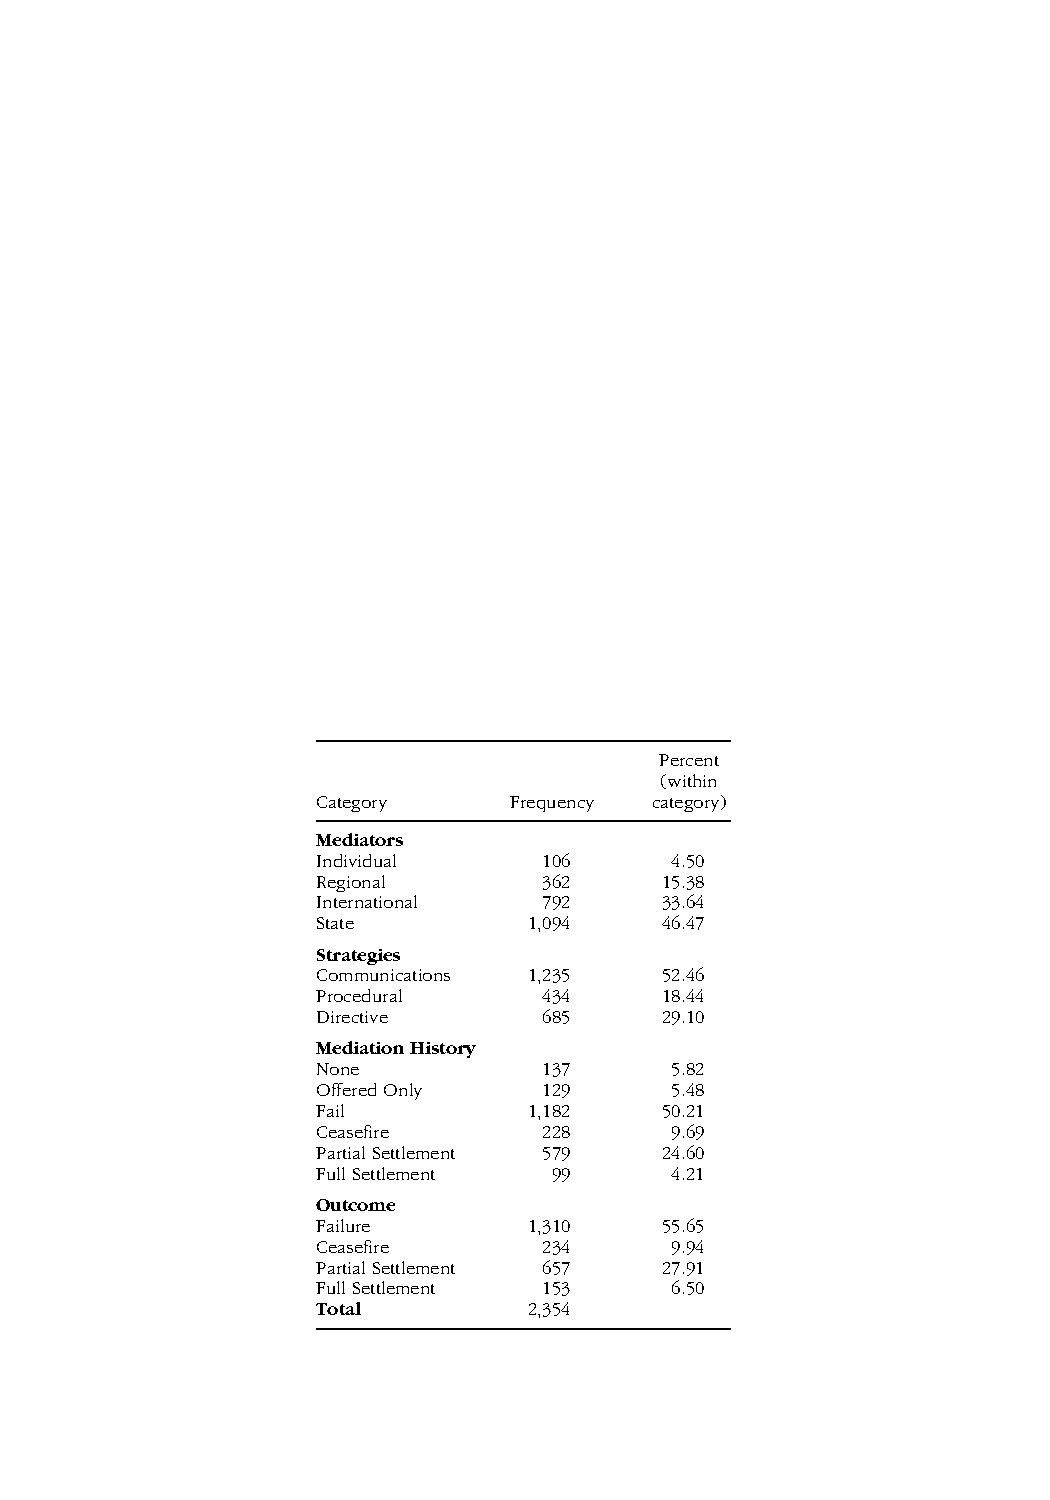
\includegraphics[scale=1]{PDF-IMG/table_mad.pdf}

\caption{Dataset Summary (Adopted from \citet{bercovitch2006}}

\label{tbl:tmad}
\end{table}
\end{center}

\subsection{Miscellaneous issues}
\label{sec:miscissues}
The literature is full of issues and factors affecting third party intervention. For example, factors affecting the process of intervention is that a mediator can act formally or informally, be invited to the conflict or not, intervene independently or on behalf of an organization, have interest in the outcome or in the process of intervention, be inclined toward one party or the other, and be consultative or directive in the intervention \citep{lewicki1992}. Furthermore, mediation history can also have an effect on a new intervention attempt \citep{bercovitch2006}. A study by \citet{carnevale2005} addresses the element of time. They found that time pressure affects the mediator to be aggressive in intervening and to use pressuring tactics. Other studies on the effectiveness of third party intervention suggest factors that influence the success of specific situations. For instance, if an uninvited third party intervenes, \citet{murray1983} specifies three important factors for mediation efficiency: dispute maturity, disputants' relationship, and intervention timing. Other issues raised by different researchers include culture, power asymmetries, conflict ripeness, number of third parties, third party authority, bias, and consistency \citep{fisher2001}.

Another aspect of mediation is strategy. The range of strategies a mediator can undertake is immense. \citet{regan1996} suggests three basic strategies of intervention within intrastate conflicts: military, economic, or mixed. \citet{young1972} discusses four intermediary functions: informational, tactical, supervisory, and re-conceptualization. In another study on successful mediation, \citet{bercovitch1991} outline different strategies that can be adopted by a third party: conciliation-facilitation, procedural, directive, substantive, and supervisory. The authors explain each of these strategies and assess their impact based on a range of historical conflicts. While these studies emphasize specific strategies, other approaches provide a more generic context, referred to as intervention styles. For instance, \citet{bartunek1975} organize intervention techniques into two broad styles: content form and process form. Another wide classification is that of Touval and Zartman, who categorize all intervention approaches as communication, formulation, or manipulation strategies \citep{bercovitch1993}.  \citet{bercovitch2006} suggest that all strategies can be grouped into communication, procedural, or directive strategies.

\subsection{Third Party Modeling}
\label{sec:tpmodel}
Many studies in the literature tackle third party intervention in the context of a specific historical conflict or set of conflicts such as the work by \citet{regan1996,bercovitch1991,dixon1996}.  For instance, the research by \citet{regan1996} on success conditions for third party interventions focuses only on intrastate conflicts and analyzes the conflicts occurred during the period between 1944 to 1994 (Table \ref{tbl:reganset}). The author suggests a regression model based on the dataset he gathered as illustrated in Fig \ref{fig:regansnap}.  The author emphasizes three intrastate conflict types: ethnic, religious, and ideological. Moreover, the regression model took into account other factors affecting the intervention such as the type of conflict, number of causalities, intervention type, and intervention target.
Other attempts to formally model third party intervention based on particular conflicts include the research by \citet{carment1996,HipelRami}. Although most third party modeling based on historical conflicts use regression analysis \citep{regan1996,dixon1996}, the latter two studies use game theory based models. In addition, \citet{fisher2001,lewicki1992} discuss different conceptual and descriptive models for third party intervention. Lastly, a standard conflict model of third party intervention is suggested by \citet{siqueira2003}.



\begin{center}
\begin{figure}[H]
\centering
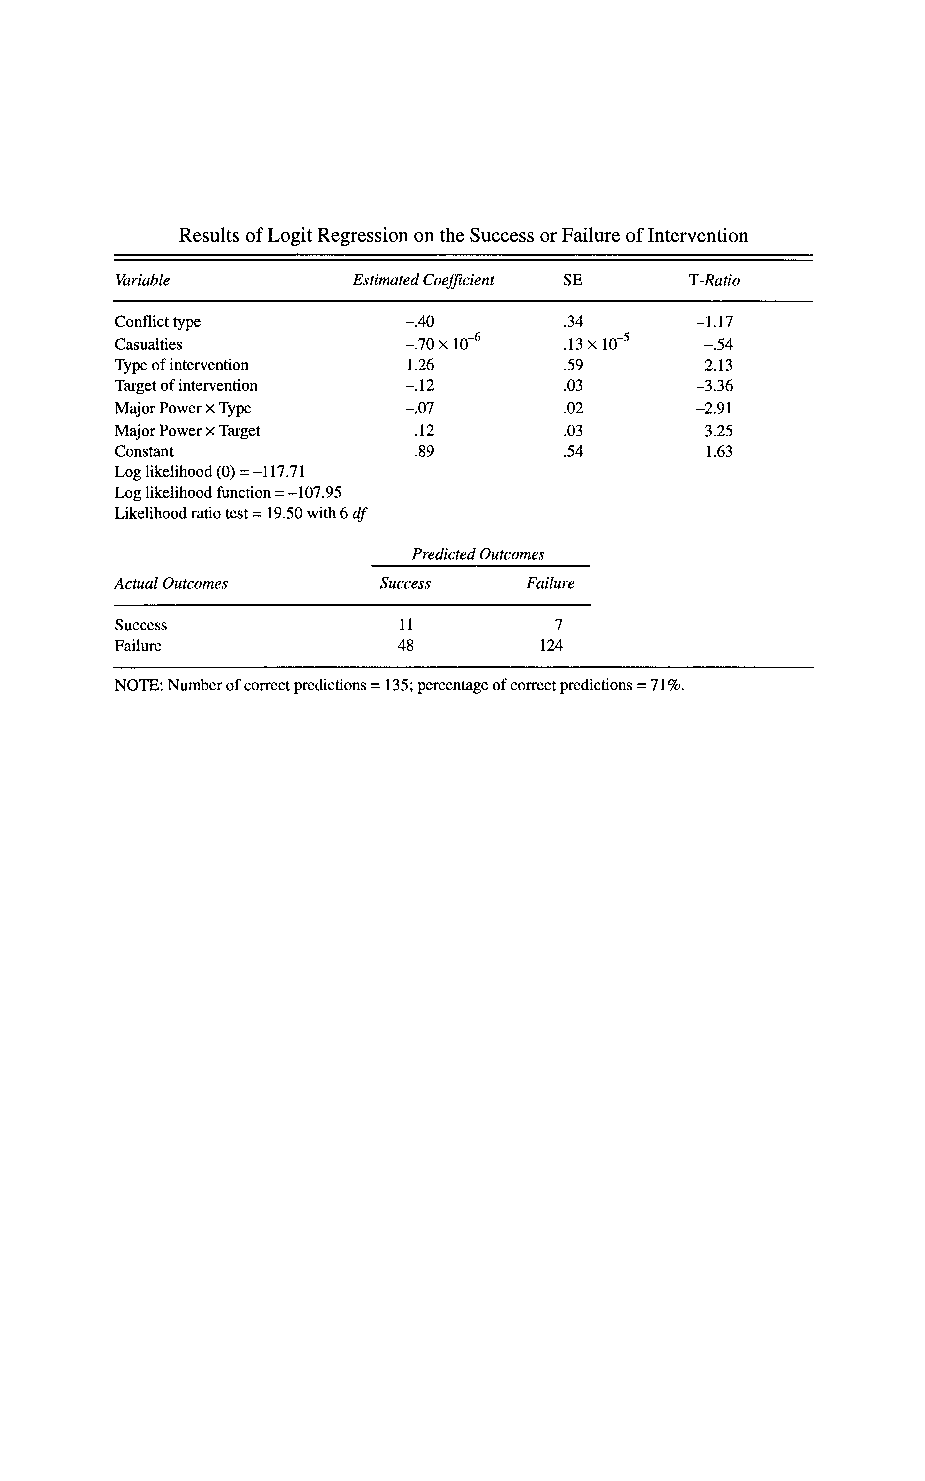
\includegraphics[scale=1]{PDF-IMG/Regan_snap.pdf}

\caption{A snapshot of the regression model by \citet{regan1996} with the results applied to the study dataset}

\label{fig:regansnap}
\end{figure}
\end{center}

\begin{center}

\begin{table}[H]
\centering
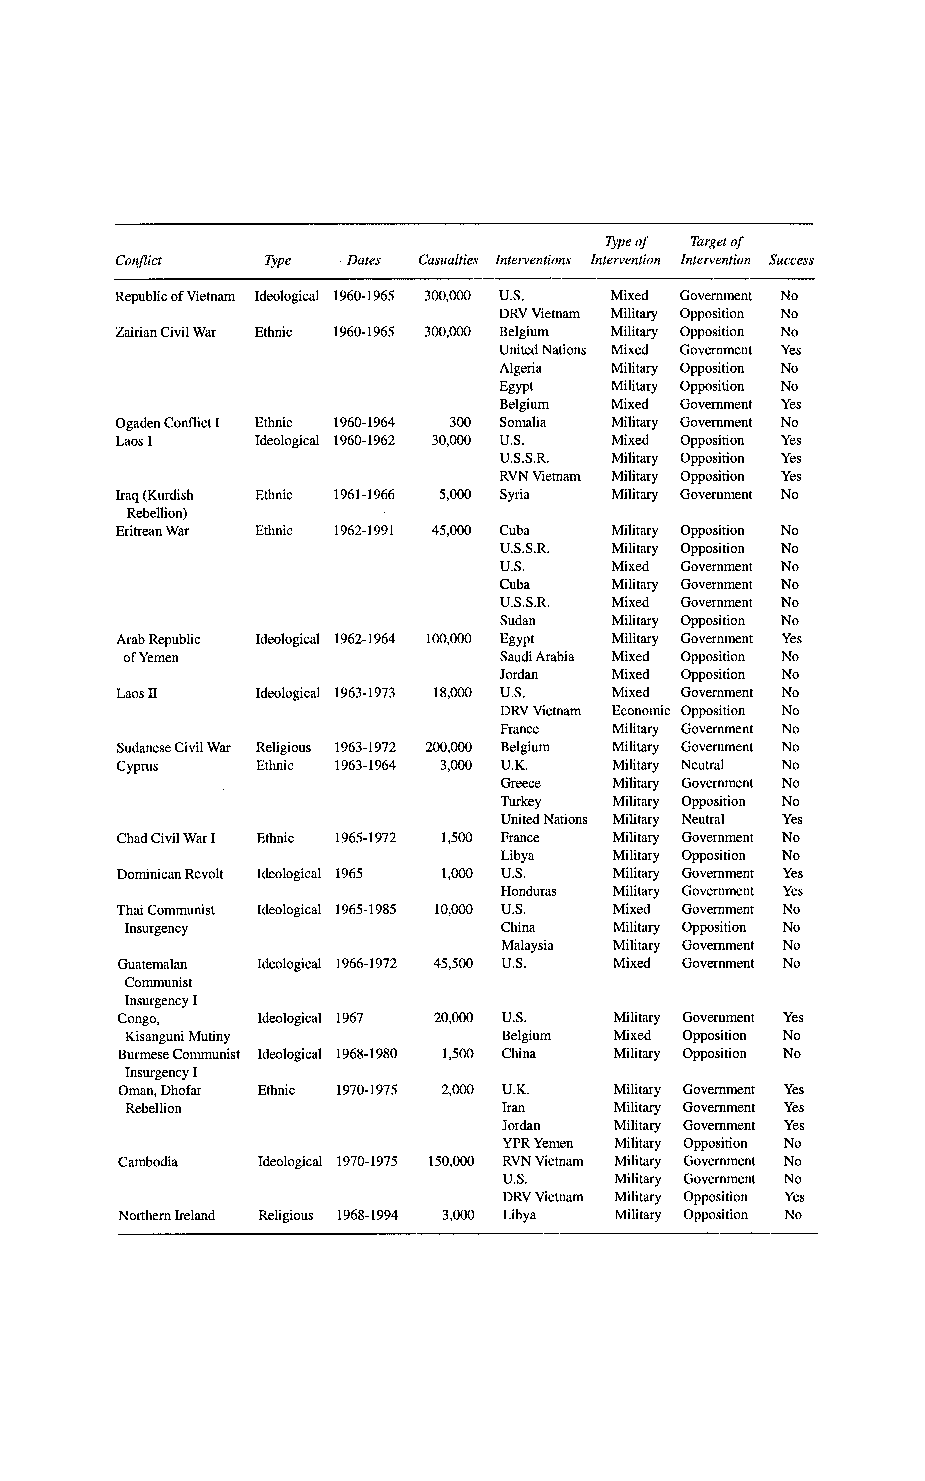
\includegraphics[scale=1]{PDF-IMG/Regan_set.pdf}

\caption{A dataset segment of the Intrastate Conflicts used in Regan's study (Table adopted from \citet{regan1996}}

\label{tbl:reganset}
\end{table}

\end{center}


A study by \citet{sakamoto2005} illustrates an approach to incorporate third party intervention in conflict modeling using GMCR. The research suggests three roles a third party can play (explained in subsection 2.1.2 of this report) and developed a conflict management procedure for them. Fig \ref{fig:sakamato_flow} below illustrates the authors' conflict management approach with the intervention of a third party.

\begin{center}
\begin{figure}[H]
\centering
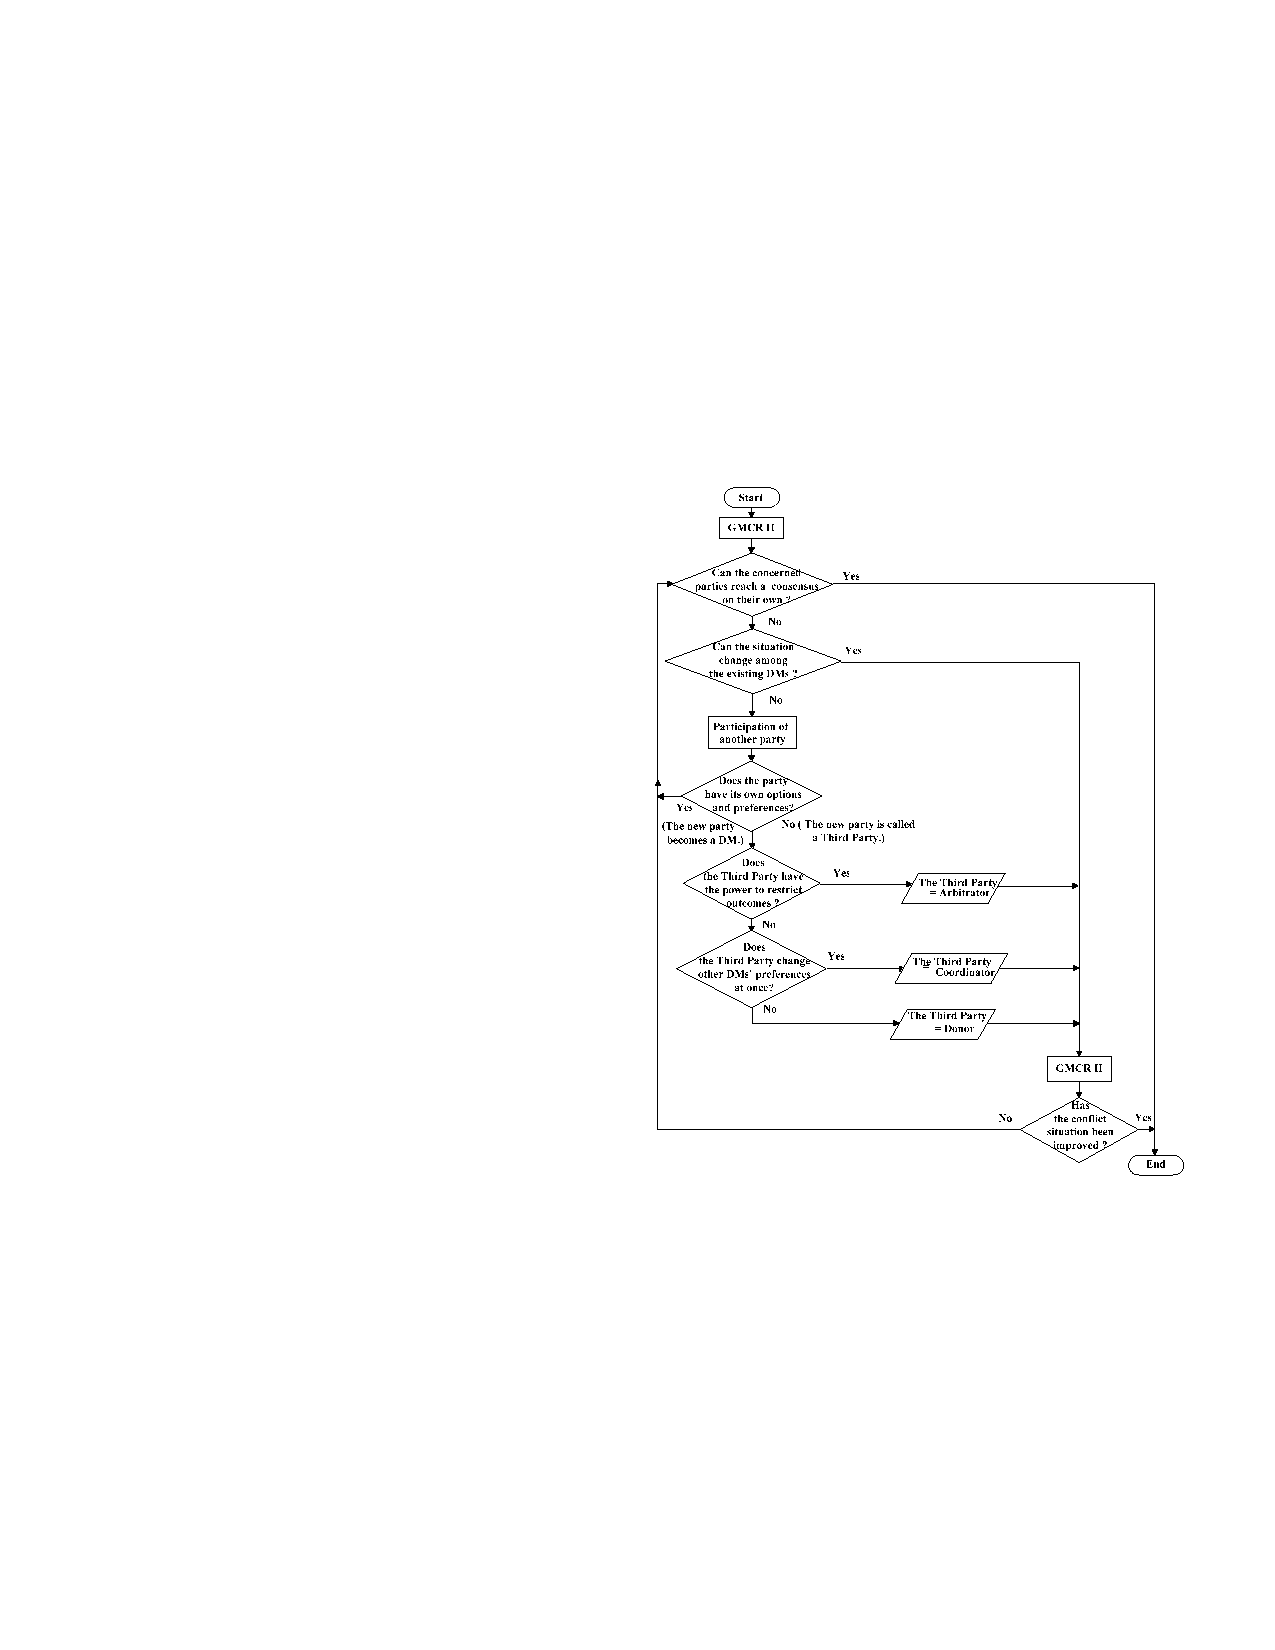
\includegraphics[scale=1]{PDF-IMG/sakamato_flow.pdf}

\caption{Chart developed by \citet{sakamoto2005} to illustrate conflict management with a third party}

\label{fig:sakamato_flow}
\end{figure}
\end{center}

A comprehensive study by \citet{bercovitch2006} investigates in depth the success factors of third party intervention. The authors focus on mediators' identities, strategies, and mediation history to predict the outcome of mediation. According to the authors, mediators can be classified according to four categories: individuals, states, regional organizations, and international institutions. After discussing each category, the authors claim that in low intensity conflicts, state and regional mediators are more likely to be successful. However, they are less likely to be successful in high intensity conflicts. International mediators are likely to be effective in high intensity conflicts and individuals are unlikely to be successful in all conflict types.
On the other hand, the authors suggest that mediation strategies include communication-facilitation, procedural, and directive strategies. Similarly, the authors make some hypotheses after explaining each of the strategies. They claim that directive strategies are most likely to be successful in high intensity conflicts but not in low intensity conflicts. Procedural strategies are mostly successful in low intensity conflicts. Tables \ref{tbl:MEDIATOR_TYPE} and \ref{tbl:MEDIATOR_STR} are summaries derived from the research hypotheses in the study. 

\begin{center}

\begin{table}[H]
\centering
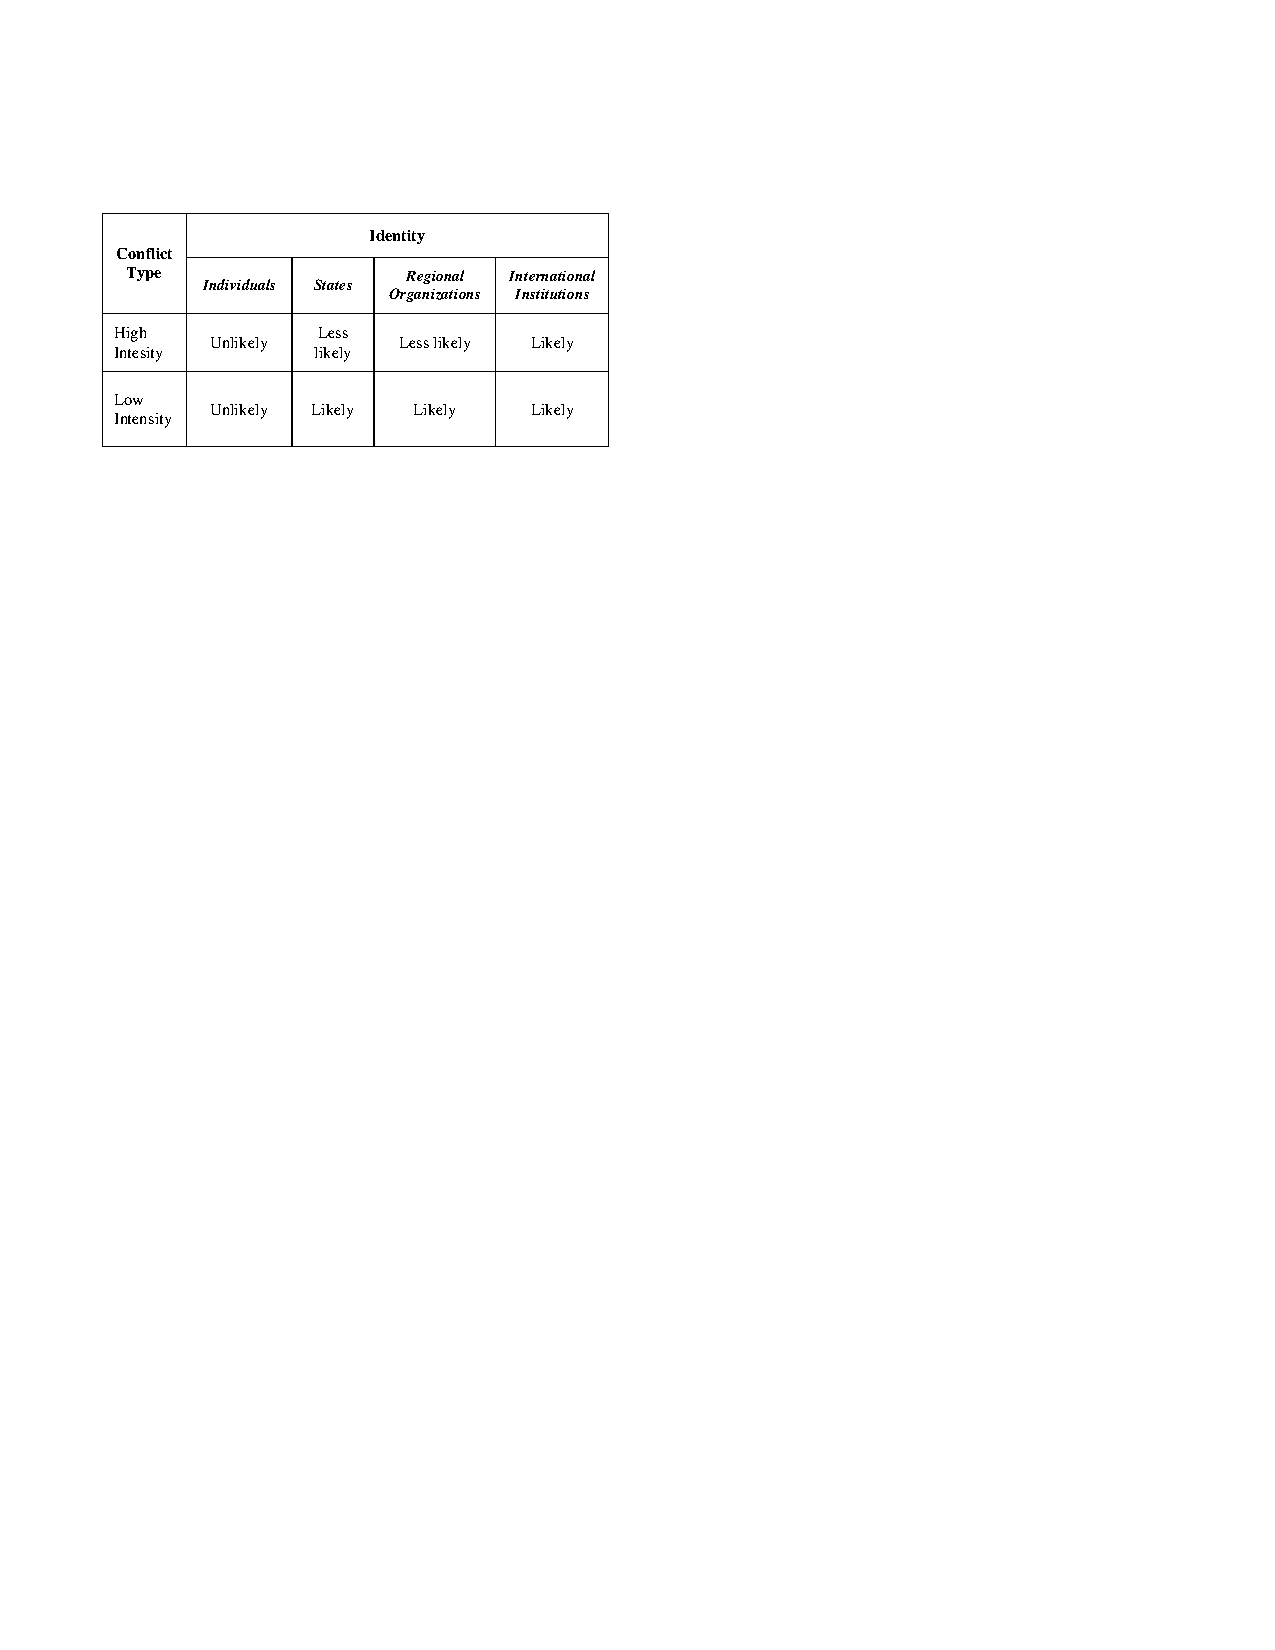
\includegraphics[scale=1]{PDF-IMG/MEDIATOR_TYPE.pdf}

\caption{Mediator type and likelihood to be successful}

\label{tbl:MEDIATOR_TYPE}
\end{table}

\end{center}

\begin{center}

\begin{table}[H]
\centering
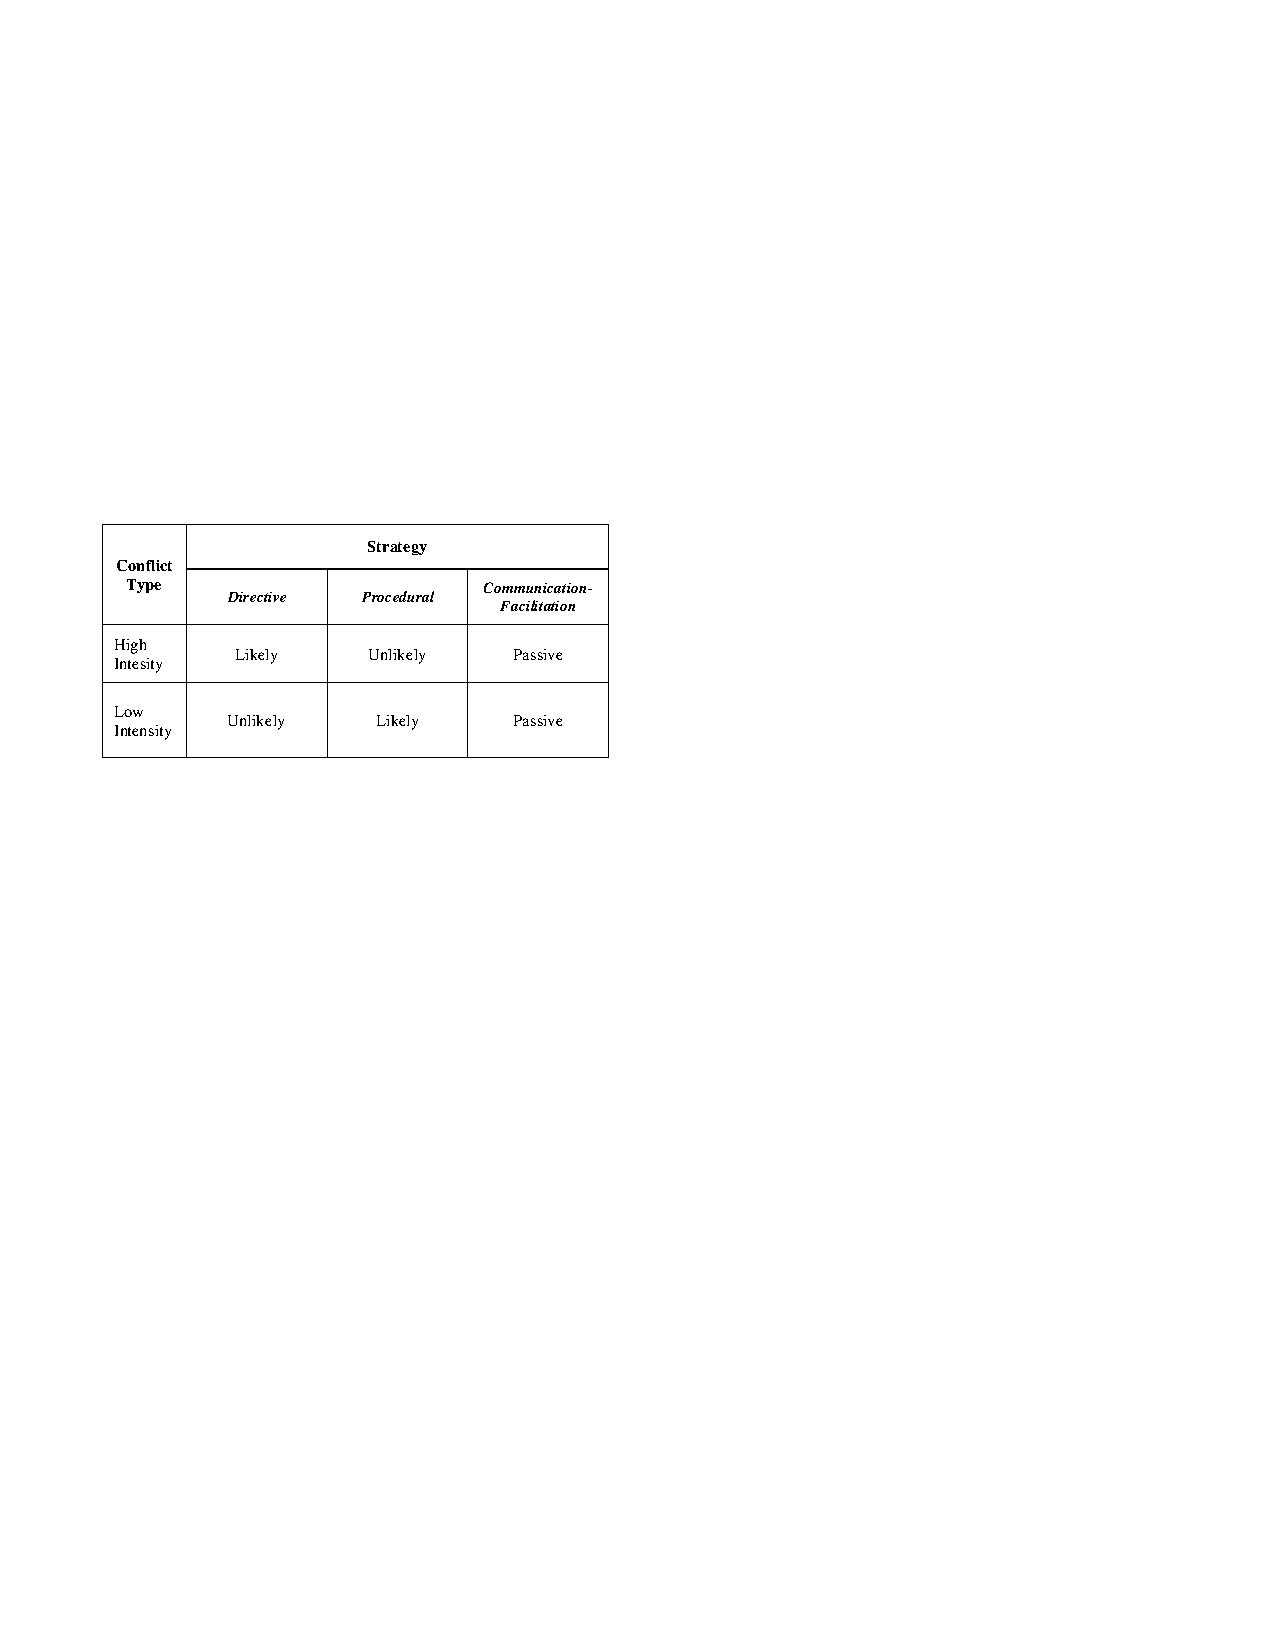
\includegraphics[scale=1]{PDF-IMG/MEDIATOR_STR.pdf}

\caption{Mediator strategy and likelihood to be successful}

\label{tbl:MEDIATOR_STR}
\end{table}
\end{center}

\section{Models and Approaches}
\subsection{General models}


red book
The most popular theory of argumentation is that of Eemeren and Grootendorst's (2004) [pg. 68], another is the Douglas Warton studies of argumentation (1989, 1996) [pg. 68]. Legal argumentation is studies through case-based and logic-based approaches as well as argument-scheme approach. [pg. 68]. On the other hand, computational models for multi-agent negotiation and argumentation-based systems are used for artificial intelligence and multi-agent research. [pg. 68]. Some negotiation studies in the 1990s that emphasized processing of information and heuristic aspects of decision-making constitute Shakun (1988), Nisbett and Ross (1980), Taylor and Crocker (1981), Payne et al (1992), Alderfer (1987).

Most early research in negotiation used primarily artificial environments such as lab experiements, scenarios and sociological methods such as interviews and questionnaries [pg. 69]. The novel trends called for authentic data obtained through face-to-face recordings, e-negotiations in different activities such as business negotiation, bargaining, task management etc. This allows adequate analysis such as discourse analysis, activity-based-communication analysis, conversation analysis, etc.[pg. 69]

Information systems for negotiation modeling require characterization of social interactions with its goal of reaching a desired resolution [pg. 398]. Previous information systems undermined the need for third party role in negotiation. 

Negotiation began to be conducted electronically with the advent of internet as a communication too. [pg. 6]. This allowed regulation and monitoring of the negotiation for analysis. Various negotiation models were developed from fields of engineering, communication research, management science, and psychology [pg. 6]. The negotiation process can be defined as "(...) the interaction that occurs between the parties before the outcome (...)" (Thompson, 1990, p.516) [pg. 121]. The process is highly interdependent where decision-making depends on the interactions betweens DMs. This is reflected in the structure of previous negotiation support systems. [pg. 121]

The various methods to analyze negotiation processes rely on different interactions between DMs [pg. 121]. One qualitative strategy to analyze negotiations is ``Coding" by categorizing, paraphrazing, or summarizing the text. This data can further be subjected to other quantitative analyses. Another strategy is ``Analysis" by revealing and uncovering meanings of the text. This leads to augmented material and reconstructing the structure of the text [pg. 121].

Group Decision Support Systems (GDSS) have been used for over 30 years for various reasons, including providing anonymity (Jessup and Tansik, 1991; Valacich et al., 1992a,), increasing group productivity (Jessup and Valacich, 1993), visual interactive modeling (Ackermann and Eden, 2001a), and enabling collaborative working (Agres et al., 2005; Briggs et al., 2003) [pg. 285]. In recent times, there are trends in the collaboration engineering arena (de Vreede et al., 2003; de Vreede and de Bruijn, 1999; van den Herik and de Vreede, 2000) to focus GDSS application in negotiations between DMs to reach a desired resolution [pg. 285].

There are quantitative as well as qualitative approaches for providing group negotiation support. The quantitative approaches are graph models for conflict resolution (Fang et al., 1993), Game Theory (von Neumann and Morgenstern, 1944), and others that view negotiation within a game theory framework (Bennett et al., 1997; Bennett, 1980) and through the use of Negotiation Support Systems (Meister and Fraser, 1994). On the other hand, the qualitative approaches seek out ``Getting to Yes" (Fisher and Ury, 1982) and ``Building Agreement" (Fisher and Shapiro, 2007) with emphasis on 'reaching agreements' and 'changing thinking' instead of mathematically optimum solutions [pg. 285]. 

The first, and best known computer supported GDSS was 'Group Systems' (Dennis et al., 1988; Nunamaker et al., 1991). 'Meeting Works' is another GDSS based on a decision analysis framework (Lewis, 1993). A third GDSS focusing on negotiation is called 'Group Explorer' which is based on the Strategic Options Development and Analysis (SODA) methodology (Ackermann and Eden, 2001a)  [pg. 286, 287].

A DSS has to be user-oriented by allowing the DM to understand and formalize preferences while being problem-oriented by defining the problem structure, searching for a resolution, and conducting sensitivity analysis [pg. 363]. 

blue book
In a conflict situation, when other methods have failed at terminating the conflict, third party mediation is proposed  due to the imminent need for resolution [pg. 21]. However, used as a last resort, mediation is likely to happen in high intensity and complex conflicts. These conflicts rarely lead to a resolution without compromise on the part of one or more DMs involved. Therefore, agreements between DMs likely cover a limited segment of the issues in dispute and are short-lived (Gartner and Bercovitch, 2006) [pg. 21].

The ``Protracted Conflict Crisis model" was developed to support the notion that mediation is most likely to occur in crises during intense international events (Breecher and James, 1988:43) [pg.224].      

Negotiation versus mediation [pg. 172]
Although functionally equivalent, there are key procedural differences between negotiation and mediation, resulting in different sociopolitical implications for the DMs involved.

Mediation is a form of peaceful third-party intervention in conflicts for joint decision-making where the outsider has some control over the process and outcome, but the ultimate power to make decisions rests with the parties directly involved (Moore, 1986) [pg. 5]. It entails the disputants seeking assistance or accepting help from a person, group, state, or an organization to influence their behaviour, without the need for physical force or the need for legal intevention (Bercovitch, 1992: 8) [- I paraphrased the last sentence. You can quote the actual definition if you want.] [pg. 6]

21st cent book
Mediation is one of the most important methods used in international conflict resolution. Third-party mediation is usually employed in the following situation: 1. complex conflicts with no imminent resolution; 2. the DMs are unable to resolve the conflict on their own; 3. the social and political costs are mounting; 4. the DMs demonstrate willingness for diplomacy and cooperation [pg. 32].

Conflict resolution is not about eliminating conflicts, but rather accepting it and recognizing formal or informal activities undertaken by the DMs or mediators, in order to limit and reduce potential violence. The goal is to achieve an understanding and agreement to dictate future dealings with the opponents and resource allocation.  [pg. 1]

Various approaches to mediation: purely scholary studies, reflections of mediators, policy implications, proposals for academics to act as third-parties in mediations [pg. 36]

Among all methods of internation conflict resolution, negotiation is frequently tried as the first [pg. 19]. It aims to reach an agreement without use of violence and through joint decision-making by the DMs in a conflict [pg. 20]. It is a tool that requires voluntary involvement by the DMs and provides an equal platform for the DMs to agree, disagree, or modify the ultimate resolution of the conflict [pg. 8]. This can possibly lead to deadlocks and stalling in the process without outside intervention. [pg. 8]

Traditional approaches to conflict 
Power-based mediation - used during the Cold War and aimed at short-term agreements without consideration for future economy, state failure etc. that are important in modern conflicts [pg. 8]. 

New approaches: Track II diplomacy (Aggestam 2002), problem-solving workshops (Kelman 1992; Burton 1972), peacebuilding and conflict prevention measures (Sambanis and Doyle 2000; Hartzell, Hoddie, and Rothchild 2001). These new approaches involve many unofficial mediators and can be used ad hoc.   



%%%%%%%%%%%%%%%%%%%%%

%----------------------------------------------------------------------

% B I B L I O G R A P H Y
% -----------------------

% The following statement selects the style to use for references.  It controls the sort order of the entries in the bibliography and also the formatting for the in-text labels.
\bibliographystyle{apalike}
% This specifies the location of the file containing the bibliographic information.  
% It assumes you're using BibTeX (if not, why not?).
\cleardoublepage % This is needed if the book class is used, to place the anchor in the correct page,
                 % because the bibliography will start on its own page.
                 % Use \clearpage instead if the document class uses the "oneside" argument
\phantomsection  % With hyperref package, enables hyperlinking from the table of contents to bibliography             
% The following statement causes the title "References" to be used for the bibliography section:
\renewcommand*{\bibname}{References}

% Add the References to the Table of Contents
\addcontentsline{toc}{chapter}{\textbf{References}}

\bibliography{uw-ethesisB}
% Tip 5: You can create multiple .bib files to organize your references. 
% Just list them all in the \bibliogaphy command, separated by commas (no spaces).

% The following statement causes the specified references to be added to the bibliography% even if they were not 
% cited in the text. The asterisk is a wildcard that causes all entries in the bibliographic database to be included (optional).

%\nocite{*}

\end{document}
